


\section{Architecture}
\label{sam-arch}





% figure, 3 mechanisms: abstractions (via history table), 
Figure~\ref{fig-samc} depicts the three levels of SAMC: sound
exploration mechanisms, reduction policies, and protocol-specific
rules.  SAMC is built on top of sound model checking foundations such
as DPOR~\cite{Flanagan+05-Dpor, Godefroid+96-Dpor} and
symmetry~\cite{Clarke+98-SymReduct, Prasad+00-SymBasedMc}.  We name
these foundations as mechanisms because a dmck must specify
accordingly what events are dependent/independent and symmetrical,
which in SAMC will be done by the reduction policies and
protocol-specific rules.






\begin{figure}[t]

\centerline{
%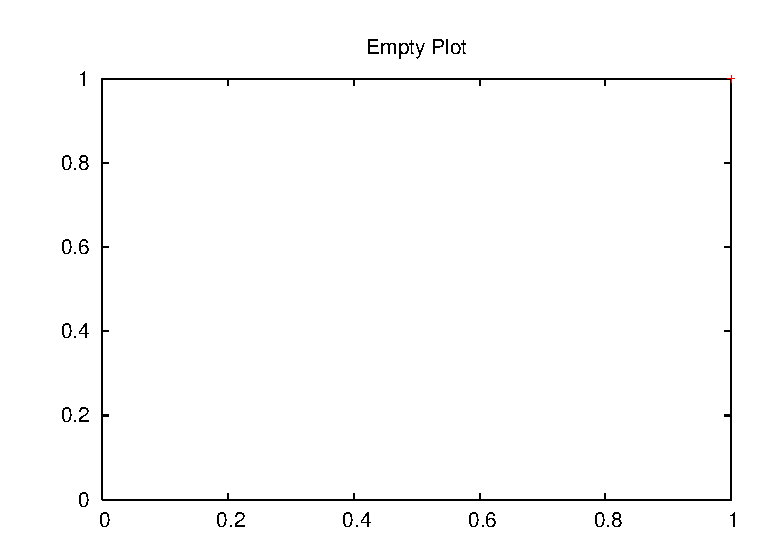
\includegraphics[height=1.4in]{F/empty.eps}
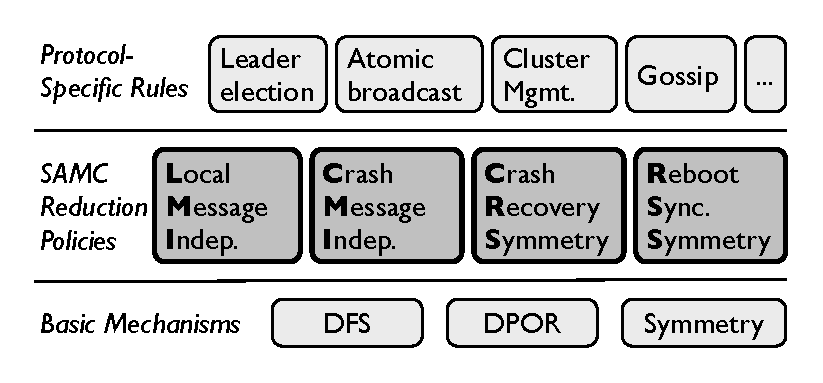
\includegraphics[height=2in]{F/samc/samc.eps}
}
\vminfive
\mycaption[SAMC Architecture]{fig-samc}{SAMC Architecture}{}
%\vminfive
\end{figure}

 % ------ fig samc

% 4 approaches and benefits
Our main contribution lies within our four novel {\em semantic-aware
  reduction policies}: local-message independence (LMI), crash-message
independence (CMI), crash recovery symmetry (CRS), and reboot
synchronization symmetry (RSS).  To the best of our knowledge, none of
these approaches have been introduced in the literature.  At the heart
of these policies are {\em generic event processing patterns} (\ie,
patterns of how messages, crashes, and reboots are processed by
distributed systems).  Our policies and patterns are simple and
powerful; they can be applied to many different distributed systems.  Testers
can extract the patterns from their target protocols (\eg,
leader election, atomic broadcast) and write protocol-specific
rules in few lines of code.

In the next section, we first present our four reduction policies
along with the processing patterns.  Later, we will discuss ways to
extract the patterns from target systems (\sec\ref{sam-extract}) and
then show the protocol-specific rules for our target systems
(\sec\ref{imp-targets}).


